\chapter{Optimizing the synthesis of monodisperse colloidal spheres}
\label{ch:synthesis}

\section{Introduction}

The earliest references of emulsion polymerization date back to 1909 \cite{bayer1909,finch03}
to a patent awarded to Felix Hoffmann and co-workers at Farbenfabriken Bayer for the
polyermization of diene monomers in the form of an aqueous emulsions.
\%\% FIXME The above is actually the first time for suspension polymerization... not emulsification.
Synthesis of colloidal spheres has progressed through
intuitive leaps guided by fundamental principles of chemistry
and physics.  Quite often, the importance of particular chemical
or physical conditions to the outcome can only be gauged once
synthesis is complete, and requires multiple orthogonal measurement
techniques. Examples include measurements of the size distribution
of their particles, their surface texture, and their porosity.
Here, we explore the role of stoichiometry, initiator choice and
agitation conditions on the synthesis of
monodisperse spheres of
\num{3}-methacryloxypropyltrimethoxysilane (TPM),
a model system with increasingly widespread applications
in soft-matter research [XXX anything else?].
We employ holographic particle characterization
in tandem with conventional particle characterization
techniques to identify factors that 
influence size selection, polydispersity and surface texture.

Spheres made from  \num{3}-methacryloxypropyltrimethoxysilane (TPM) are a 
particularly useful system for colloidal studies. Their synthesis readily 
produces monodisperse spheres in a wide range of sizes through a process 
that is simpler than that for other common colloidal particles, such 
as polystyrene and silica. There is no specialized 
equipment or inert environment necessary. The particles can be made 
in a single step through an order of magnitude of sizes, from a few 
hundred nanometers to a few micrometers. However, there are many 
parameters in the synthesis that can affect the final particle that 
is produced. In this chapter we vary a selection of these conditions 
and use holographic particle characterization to observe how they affect the 
intermediate and final products of the synthesis.

\subsection{Synthesizing TPM spheres}

Our procedure for synthesizing TPM spheres is nearly identical to the
method established in section \ref{ssec:synthesizing_tpm} for producing
ideal TPM spheres, however we reiterate the procedure to underscore the
primary synthesis steps we investigated.

The spheres in this study were made through an emulsion 
polymerization process. Monomeric TPM, which is insoluble in water, 
is added to a basic environment (pH $>$ \num{9}) of ammonia in water. The 
monomers undergo hydrolysis in the water and become water soluble. 
In a basic environment, these hydrolyzed monomers form insoluble 
oligomers. As the suspension is stirred, the oligomers condense 
homogeneously into monodisperse droplets that grow as more oligomers 
form. After \num{2} hours, this process is completed and the droplets have 
reached their final size. Once the droplets are formed, the sample is heated
to \SI{80}{\degreeCelsius} and a free radical 
initiator is introduced to polymerize the droplets and form solid spheres.

The droplet formation is done in a closed vial to prevent the 
evaporation (this is the wrong word- ammonia is a gas dissolved in the water, not a liquid...)
of the ammonia and maintain the pH throughout the droplet 
formation process. This suggests that the particular container used for 
the synthesis may affect the final product, as the amount of air above 
the suspension will affect how much ammonia is left in the water and, 
therefore, the pH of the environment. To control this, we used identical 
\SI{12}{\milli\liter} vials to make \SI{5}{\milli\liter} of colloidal 
suspension in each synthesis.





\subsection{Emulsion formation}

First, we investigate the effect of varying the stir speed of the 
suspensions during droplet formation. In four identical vials with 
identical stir bars, we place \SI{15}{\milli\liter} of 
\SI{29}{\percent} ammonia followed by \SI{200}{\micro\liter} of TPM 
monomer to \SI{5}{\milli\liter} of DI water. The four samples are then stirred 
using magnetic stir plates set at \num{500}, \num{700}, \num{900}, and
\SI{1100}{\minute^{-1}} for \SI{2}{\hour}. % XXX Use rpm instead of min^{-1}?
At this point the droplets have stopped growing and they are polymerized 
by adding \num{2},\num{2}'-azobis(\num{2}-methylpropionitrile) (AIBN) and 
heating the sample to \SI{80}{\celsius} for \SI{2}{\hour}. 
%XXX Add conclusions about stir speed- surprisingly, the faster stir speed led to larger droplets...)

To probe the variables of droplet formation, we make four batches of droplets.
In each case we hold the volume of water, \SI{5}{\milli \liter} constant 
and vary the amounts of TPM and ammonia. Batches A and B each had 
\SI{100}{\micro\liter} of TPM with \si{10} and \SI{20}{\micro\liter} of 
ammonia added, respectively. Batches C and D had \SI{150}{\micro\liter}, 
again with \si{10} and \SI{20}{\micro\liter} of ammonia, respectively. 
The polymerization for all of the particles was done in \SI{0.1}{\percent} 
sodium docecyl sulfate (SDS) to avoid aggregation.
Through this, we can observe the effects of varying 
the amount of TPM and the pH on the size of the resulting droplets.
This gives 
% XXX (Add conclusions about initiator- does not seem to matter)

\subsection{Polymerization}

The polymerization of the TPM droplets can be tracked by observing the 
refractive index of the particles over time. As the droplets polymerize, 
their refractive index increases until they are fully polymerized. To track 
this, we sampled the suspension above that was stirred at \SI{1100}{\min^{-1}}
% XXX Again, rpm vs mins^{-1}
after \si{5}, \si{10}, \si{15}, \si{20}, \si{40}, and \SI{60}{\min} of 
heating and measured the particles' refractive index. 
%XXX (Add conclusions about polymerization time- only takes maybe 15 min?)

Next, we observe the effect of using different free radical initiators 
to polymerize the particles. Two water-insoluble initiators, AIBN and
\num{1},\num{1}'-azobis(cyclohexanecarbonitrile) (ACHN), and two water-soluble 
initiators, potassium persulfate (KPS) and ammonium persulfate APS), were 
used.

To compare initiators, one \SI{5}{\milli \liter} suspension of emulsion droplets is
made in a \SI{12}{\milli \liter} vial and then equally divided into five
\SI{1.5}{\milli \liter} microcentrifuge tubes. One tube was left unpolymerized. The
other four tubes were then polymerized at \SI{80}{\celsius} 
for \SI{12}{\hour} on a shaker at \SI{750}{\minute^{-1}} % XXX Again, rpm vs mins^{-1}
to prevent sedimentation.
We added a different free radical initiator to each tube and repeated the process with four
different emulsions for a total of 
\num{16} measurements to ensure that any observations were the result of the 
initiator used and not of the particular protocol used to make the emulsion.

\subsection{Characterization}


We utilize a Spheryx xSight, a commercial holographic particle characterization system,
to measure the  refractive index and diameter of our synthesized TPM spheres.
The xSight flows a colloidal sample through the optical volume of a conventional microscope
that is illuminated by a green laser. The proprietary software and hardware implemented in
the instrument yields the size and refractive index for each observed colloidal spheres and
does so in a fraction of the time we typically spend analyzing an experimental video.
Because we are only interested in collecting population statistics for the size and refractive
index of our colloidal systems, we utilize the xSight rather than our custom-built microscope.

The manufacturer recommends that the sample number density remain below 
\SI{E6}{\milli\liter^{-1}} to reduce the extent to which
holograms overlap which is consistent with our discussion in section \ref{ssec:sample_prep}.
The above emulsification polymerization process produces
a sample with a number density of \SI{E10}{\milli\liter^{-1}} therefore we
dilute each of our samples by a factor of \si{E4}.
We utilized \SI{50}{\micro \liter} xCells, the flows cells designed for the xSight,
with each flow analyzing \SI{3}{\micro\liter} of sample; this provides us with
scattering information of a few thousand colloidal spheres per sample.


\begin{figure}
    \centering
    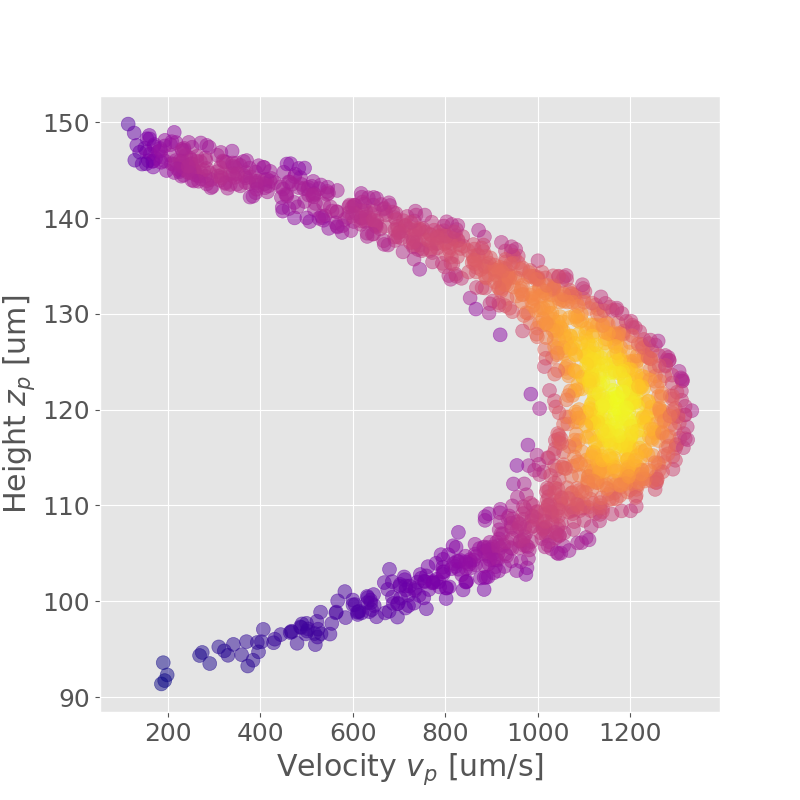
\includegraphics[width=0.9\columnwidth]{example_poiseuille}
    \caption{The recorded Poiseuille flow of particles streaming through the xCell. The
      color denotes the density of observations. \%FIXME: add color bar.}
    \label{fig:flow_prof}
\end{figure}


The flow cell is at rest while the dilute suspension flows above
the field of view producing a Poiseuille flow of fluid through the
xCell. Because the xSight records the mean $z$-position and mean 
velocity of all multiply-imaged scatterers, we are able to fit the flow
profile to a Poiseuille flow as depicted in Fig.~\ref{fig:flow_prof}
To refine the population estimates of refractive index and diameter, 
we filter the data which deviates from our parabolic fit by more 
than one median absolute deviation.

\section{Results}

\subsection{Role of Stir rate}

The results for the \num{4} polymerized and \num{4} unpolymerized
samples are summarized in Fig.~\ref{fig:stir_rate}.

\begin{figure}
    \centering
    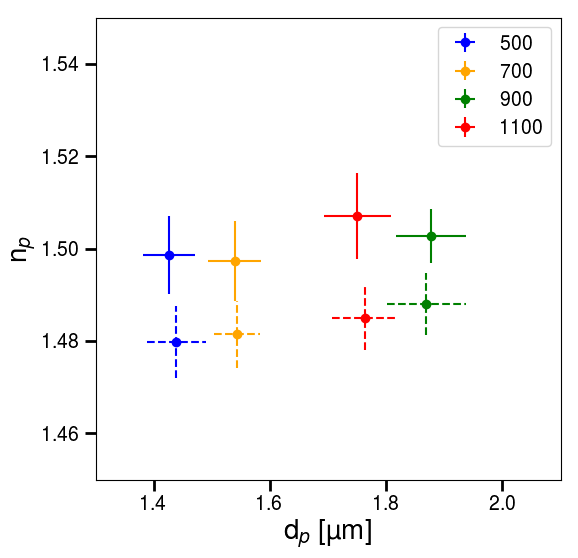
\includegraphics[width=0.9\columnwidth]{may_data_stirring_both}
    \caption{Caption}
    \label{fig:stir_rate}
\end{figure}


\subsection{Role of emulsion conditions}
\%(This title is terrible)


\begin{figure}
    \centering
    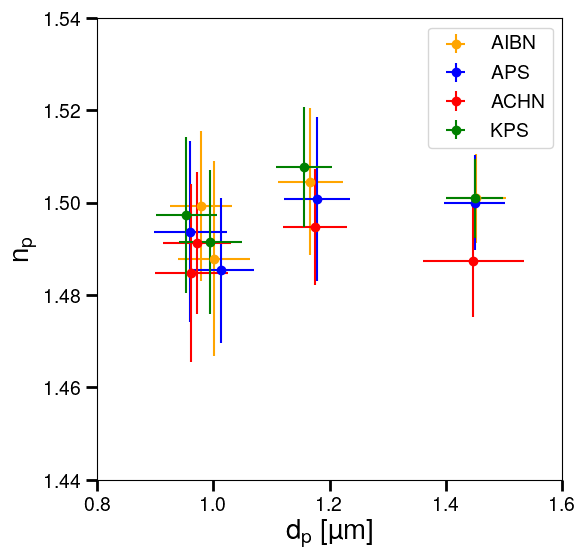
\includegraphics[width=0.75\columnwidth]{may_data_summary.png}
    \caption{The refractive index and diameter of 16 samples of 
    polymerized TPM.}
    \label{fig:initiator_data}
\end{figure}

In making the \si{16} sets of particles to look at the effect of initiator on 
the particles, we can also make observations about the effects of varying 
the amount of TPM and the pH on the size of the resulting droplets. To hold 
the pH constant, we can compare sample A to C and sample B to D. This gives 
the fairly intuitive result that increasing the amount of TPM increases the 
size of the final droplet. Holding the amount of TPM constant and varying 
the pH, which means comparing A to B and C to D, shows that increasing the 
pH of the environment during droplet formation decreases the size of the 
final droplet. This is less intuitive but perhaps not surprising, as the pH 
affects the rate at which oligomers form and therefore the rate of droplet 
formation. This leads to more nucleation sites and therefore smaller droplets 
for the same volume of material. 

Comparing batches A to C, each with \SI{100}{\micro \liter} of TPM monomer, and B to D with
\SI{150}{\micro \liter}, gives the somewhat intuitive result that increasing the amount of TPM
monomer increases the size of the final droplet. On the other hand, comparing A to B with
\SI{10}{\micro \liter} ammonia and C to D with \SI{15}{\micro \liter} ammonia shows that
increasing the pH of the environment during droplet formation decreases the size of the 
final droplet. This is less intuitive but perhaps not surprising, as the pH 
affects the rate at which oligomers form and, therefore, the rate of droplet 
formation. Increasing the pH results in more nucleation sites and therefore smaller droplets 
for the same volume of material. 

\subsection{Role of Initiator.}

Under certain conditions, TPM droplets are known to form dimpled spheres when polymerized with
the water-soluble initiators APS and KPS due to the ejection of low molecular weight oligomers
(citation- I forget which of Stefano's papers?). Therefore, one might think that TPM spheres
polymerized with these initiators would be made of on average higher molecular weight oligomers
and have a higher refractive index than pa. However, under the conditions observed here where no
dimple was formed, there was no observable difference in particle size or refractive index between
the initiators used.

\subsection{Role of Heat Bath.}


\begin{figure}
    \centering
    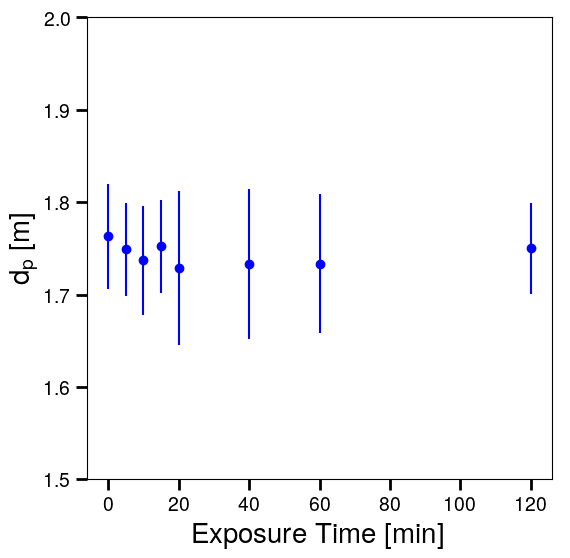
\includegraphics[width=0.9\columnwidth]{may_data_heat_bath_size_time}
    \caption{Caption}
    \label{fig:heat_size_time}
\end{figure}



\begin{figure}
    \centering
    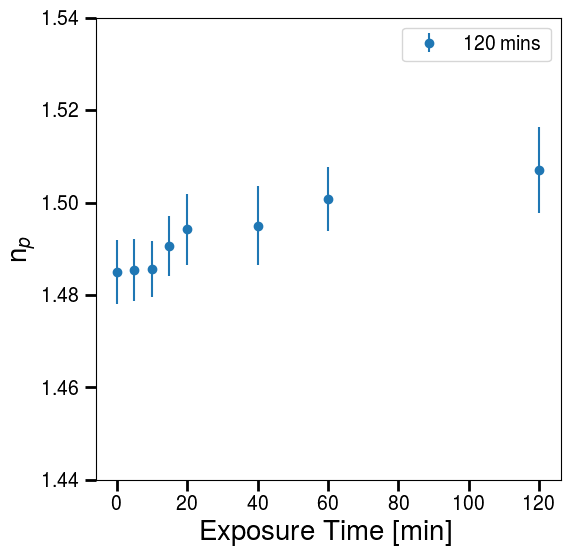
\includegraphics[width=0.9\columnwidth]{may_data_heat_bath_time}
    \caption{Caption}
    \label{fig:heat_ref_time}
\end{figure}

\section{Discussion}
